\documentclass[12pt, twocolumn]{article}
\usepackage[margin=3cm]{geometry}
\usepackage{listings}
\usepackage{graphicx}
\usepackage{float}
\usepackage{tikz}
\usepackage[justification=centering]{caption}
\usetikzlibrary{shapes.geometric,arrows}
\renewcommand{\lstlistingname}{\textbf{Program}}


%setting up flowcharts
%\tikzstyle{startstop} = [rectangle, rounded corners, minimum width=3cm, minimum height = 1cm, text centered, draw=black, fill=red!30]

%\tikzstyle{process} = [rectangle, minimum width=3cm, minimum height = 1cm, text centered, text width = 3cm, draw=black, fill=orange!30]

%\tikzstyle{decision} = [diamond,  minimum width=3cm, minimum height = .5cm, text centered, text width = 3cm, draw=black, fill=green!30]

%\tikzstyle{arrow} = [thick, ->,>=stealth]

\begin{document}

\begin{titlepage}
	\begin{center}
		
		
		% Upper part of the page. The '~' is needed because \\
		% only works if a paragraph has started.
		\vfill
		
		\textsc{\LARGE Experiment 3: Exception Processing and System Control}\\[1.5cm]
		
		\Large Adam Sumner\\[0.5cm]
		
		\Large Illinois Institute of Technology\\[0.5cm]
		
		\Large ECE 441-01\\[0.5cm]	
		% Author and supervisor
		\noindent
		\vfill
		\large \textbf{Lab Date:} February 3rd, 2015\hfill
		\large \textbf{Due Date:} February 10th, 2015
		% Bottom of the page
		
		
	\end{center}
\end{titlepage}

\section{Introduction}
The purpose of this experiment is to acquaint the student with MC68K Exception Processing, TUTOR Exception Handling, and MC68K System Controls. The student will write and execute several programs that demonstrate all three of these topics.
\section{Background}
The processor is always in one of three states: normal, exception, or halted. The normal processing state is associated with the execution of instructions. The halted state is an indication of a hardware failure. For example, if a double bus fault occurs, the processor assumes the system is no longer stable to run and halts. Only an external reset can restart a halted processor. The exception processing state is generally associated with interrupts, trap instructions, tracing, and other exceptional conditions. An exception can be generated via instruction or by an unusual condition that arises during program execution. Externally, exception processing can be forced by an interrupt or by a reset. It provides an efficient context switch so that the processor is able to handle unusual conditions\cite{m68k}. The processing of an exception occurs in four steps:
\begin{enumerate}
	\item Make a temporary copy of the status register and set it for exception processing
	\item Obtain the exception vector
	\item Save the current processor context
	\item Obtain a new context and resume instruction processing
\end{enumerate}

An exception vector is a location in memory in which there is a subroutine of instructions for the processor to execute. Each exception type requires a handler routine and its very own vector. Each vector is two words in length except for the reset vector which is located in the supervisor space of memory.
\section{Equipment/Procedure}
\subsection{Equipment}
\begin{itemize}
	\item \textsc{SANPER-1 Educational Lab Unit}
	\item Computer with TUTOR software
\end{itemize}
\subsection{Procedure}
\subsubsection{Program 1}
\begin{enumerate}
	\item Load program located in Section \ref{prog1A} in memory and initialize D0 to \$FF
	\item Execute and record results
	\item Load program located in Section \ref{prog1B} in memory and initialize D0 to \$FF
	\item Execute and record results
	\item Modify memory address \$2000 to contain the value 4AFA
	\item Type ``G \$2000" into TUTOR and record the results
	\item Load program located in Section \ref{prog1D} in memory and initialize Status Register to \$FFFF
	\item Execute and record results
	\item Load program located in Section \ref{prog1E} in memory, initialize D1 to \$0000, and D2 to \$1000 
	\item Execute and record results
	\item Load program located in Section \ref{prog1F} in memory, initialize D6 to \$3000, and D2 to \$3010 
	\item Execute and record results
	\item Modify memory address \$2000 to contain the value A000
	\item Type ``G \$2000" into TUTOR and record the results
	\item Modify memory address \$2000 to contain the value F000
	\item Type ``G \$2000" into TUTOR and record the results
\end{enumerate}
\subsubsection{Program 2}
\begin{enumerate}
	\item Load program located in Section \ref{prog2} into memory
	\item Modify memory address \$A to contain the value 0950 
	\item Load program located in Section \ref{prog2-4} into memory and execute it
	\item Reset the system and run program located in Section \ref{prog2-4} again
	\item Load program located in Section \ref{prog2-12} into memory and repeat step 3
	\item Record results
	
\end{enumerate}
\subsubsection{Program 3}
\begin{enumerate}
	\item Load program located in Section \ref{prog3} into memory
	\item Modify memory location starting at \$9 to contain the value FFFFFE
	\item Execute program and record results
\end{enumerate}
\section{Results}
Below are the recorded results from inciting a bus error, along with the results from the halted state of the \textsc{sanper-1 elu}.
\begin{figure}[h!]
\centering
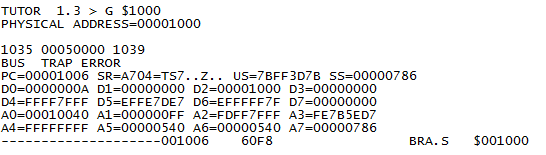
\includegraphics[width=1\linewidth]{3_2_10}
\caption{Results from Program 2 Procedure 10}
\label{fig:3_2_10}
\end{figure}

\begin{figure}[h!]
\centering
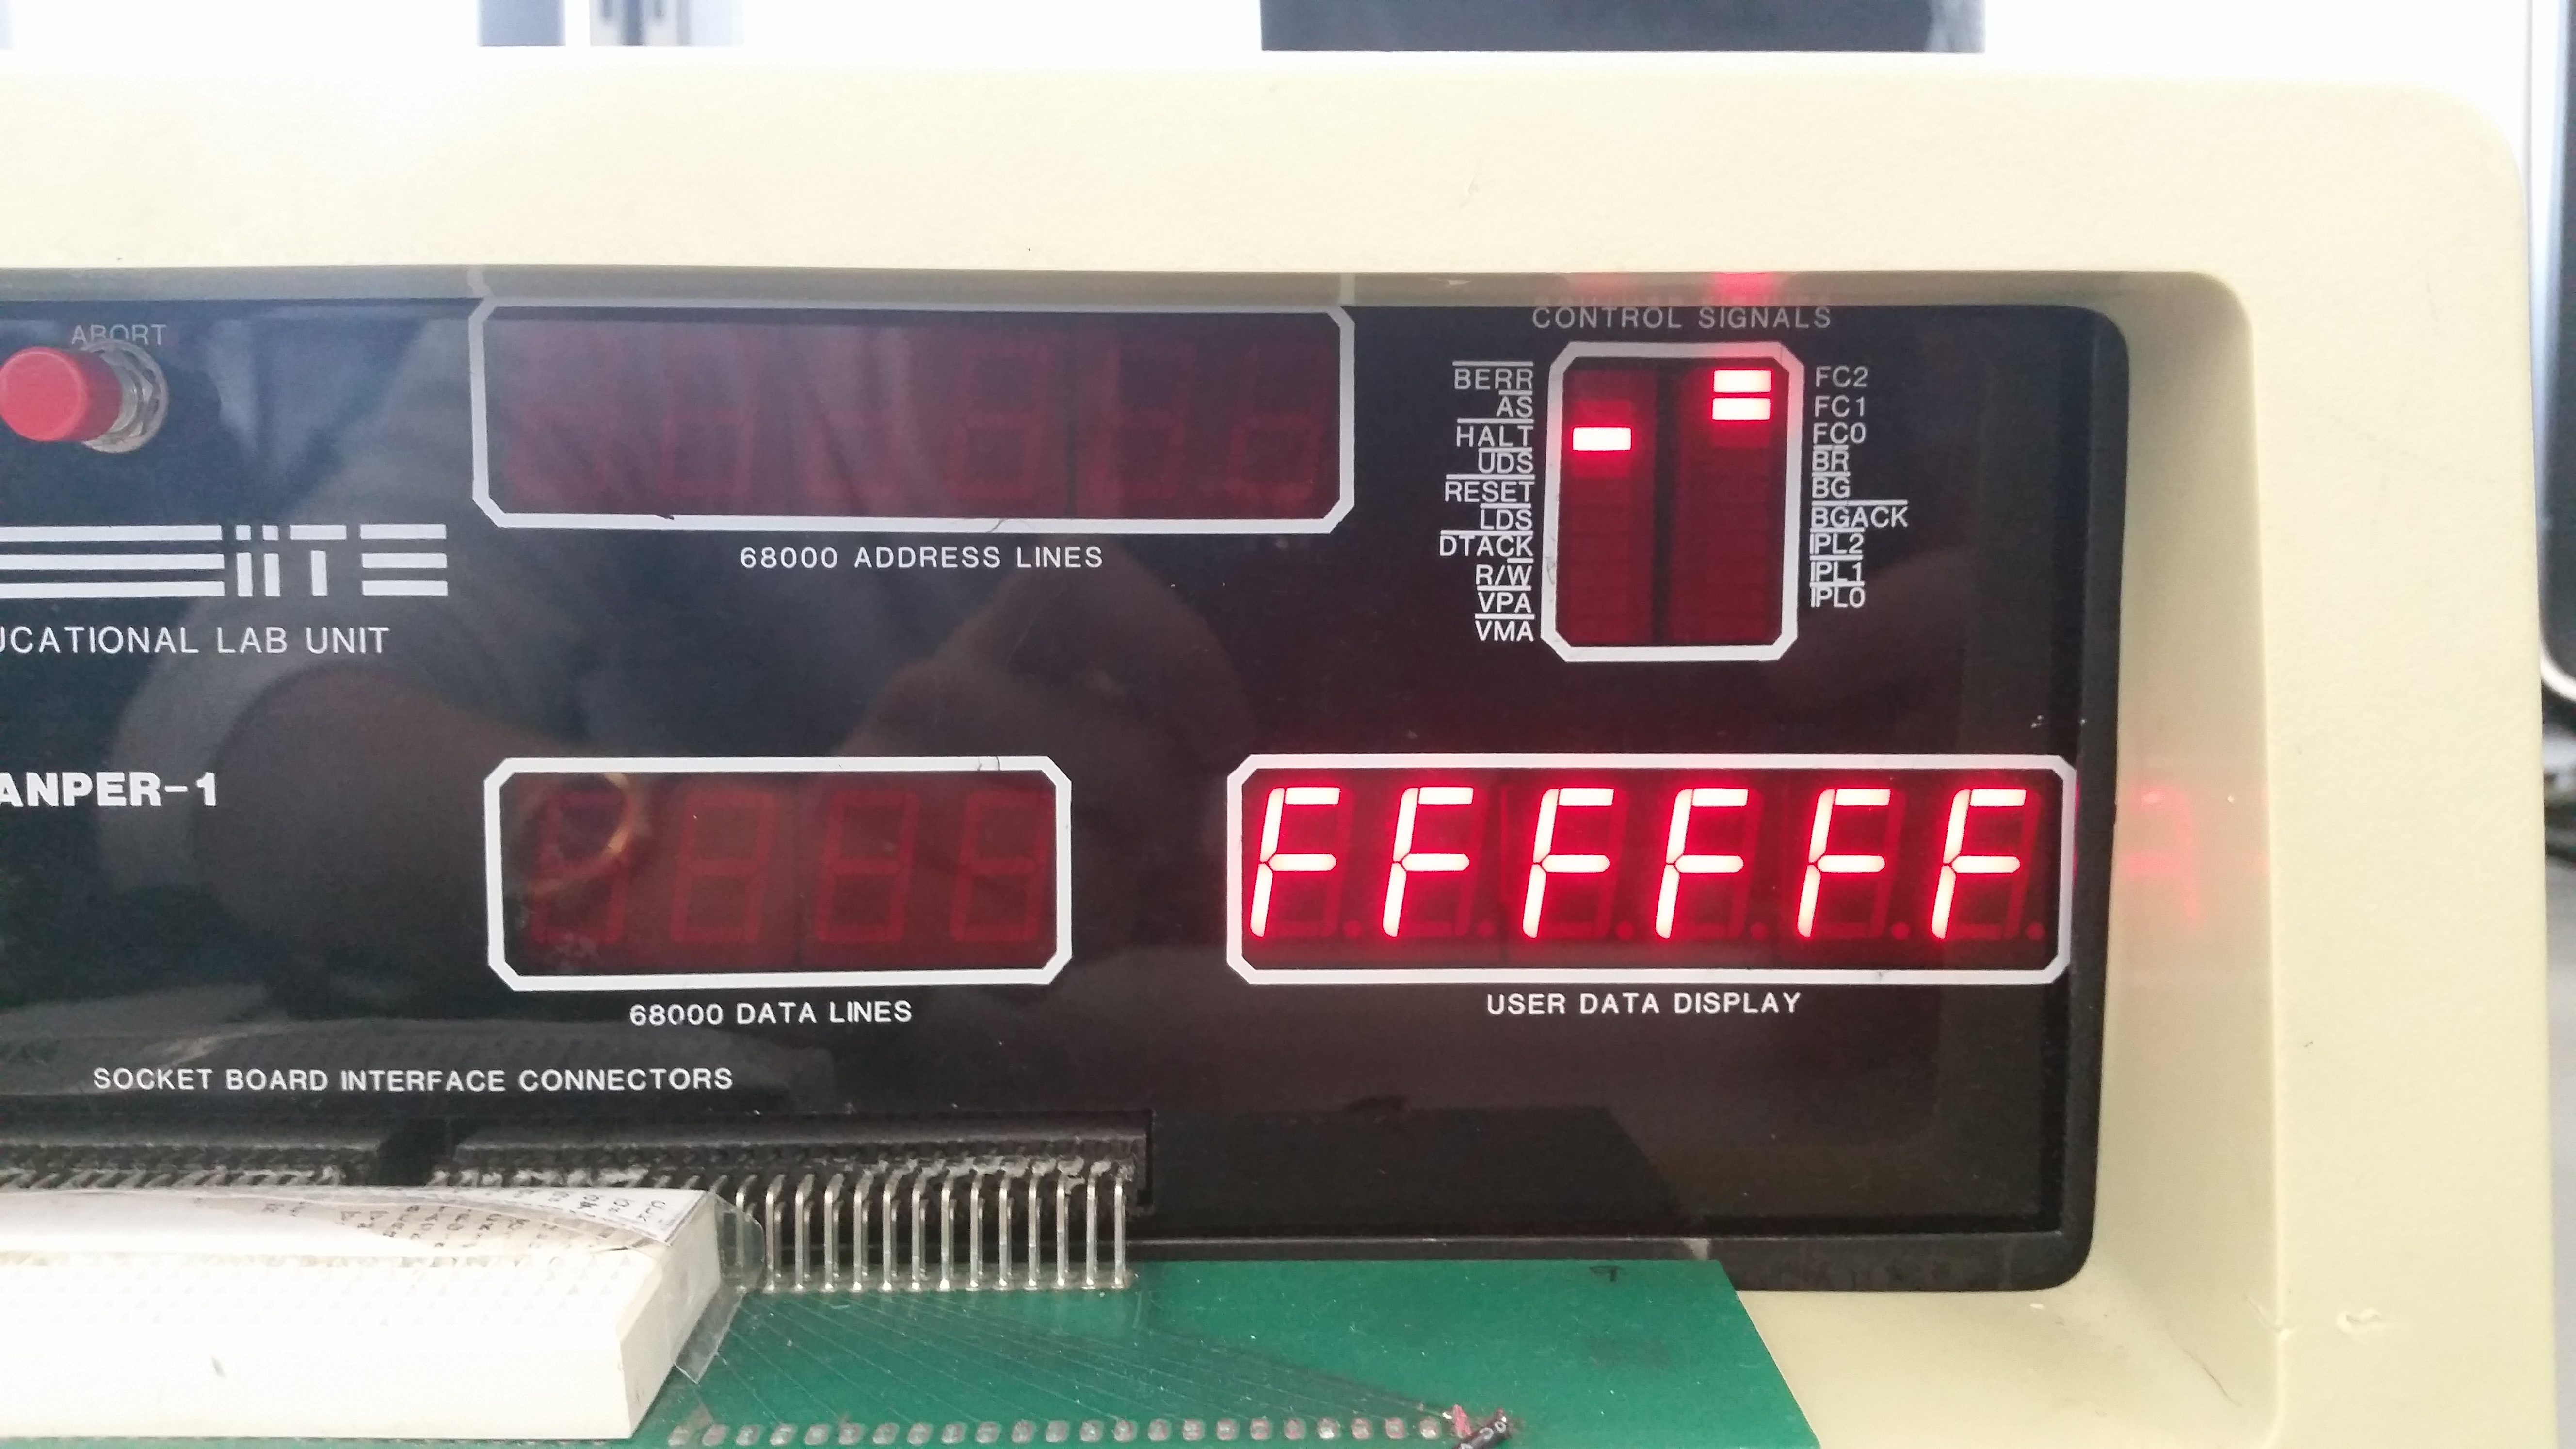
\includegraphics[width=1\linewidth]{20150203_094107}
\caption{Halted State of \textsc{sanper-1 elu}}
\label{fig:halt}
\end{figure}

\begin{figure}[h!]
\centering
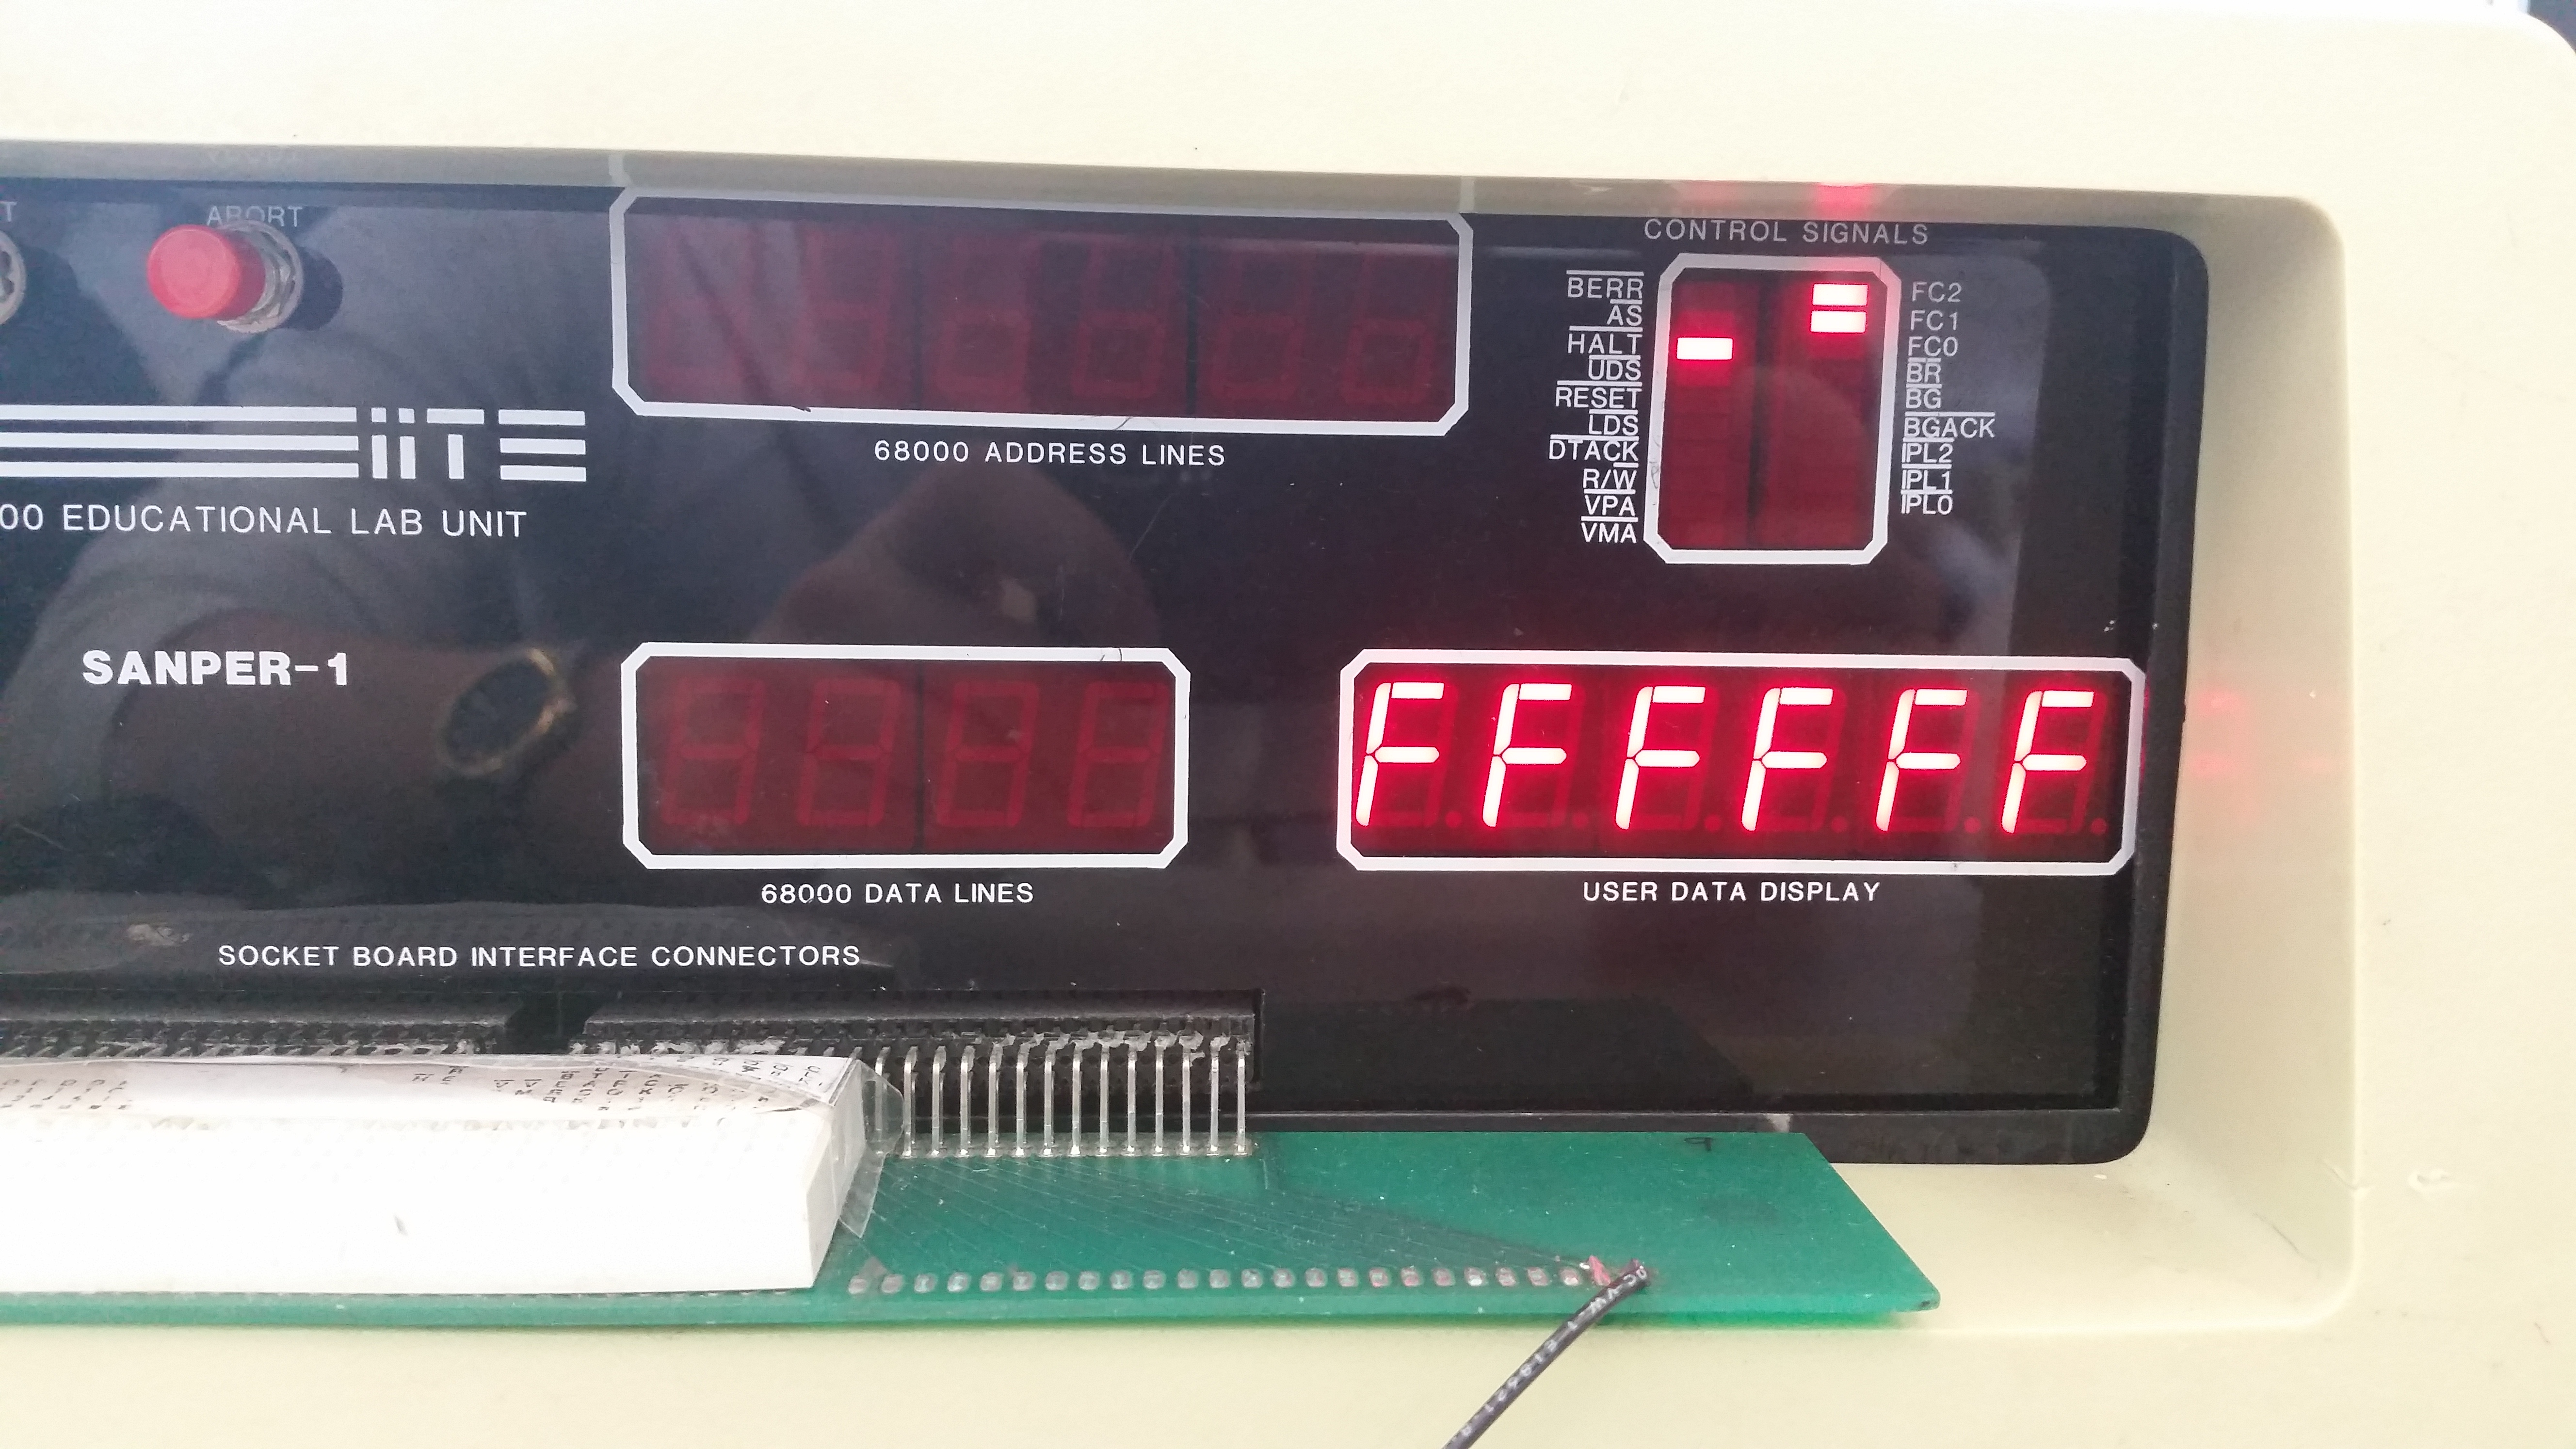
\includegraphics[width=1\linewidth]{20150203_094116}
\caption{Halted State After Pressing the Abort Button}
\label{fig:abort}
\end{figure}

\begin{figure}[H]
\centering
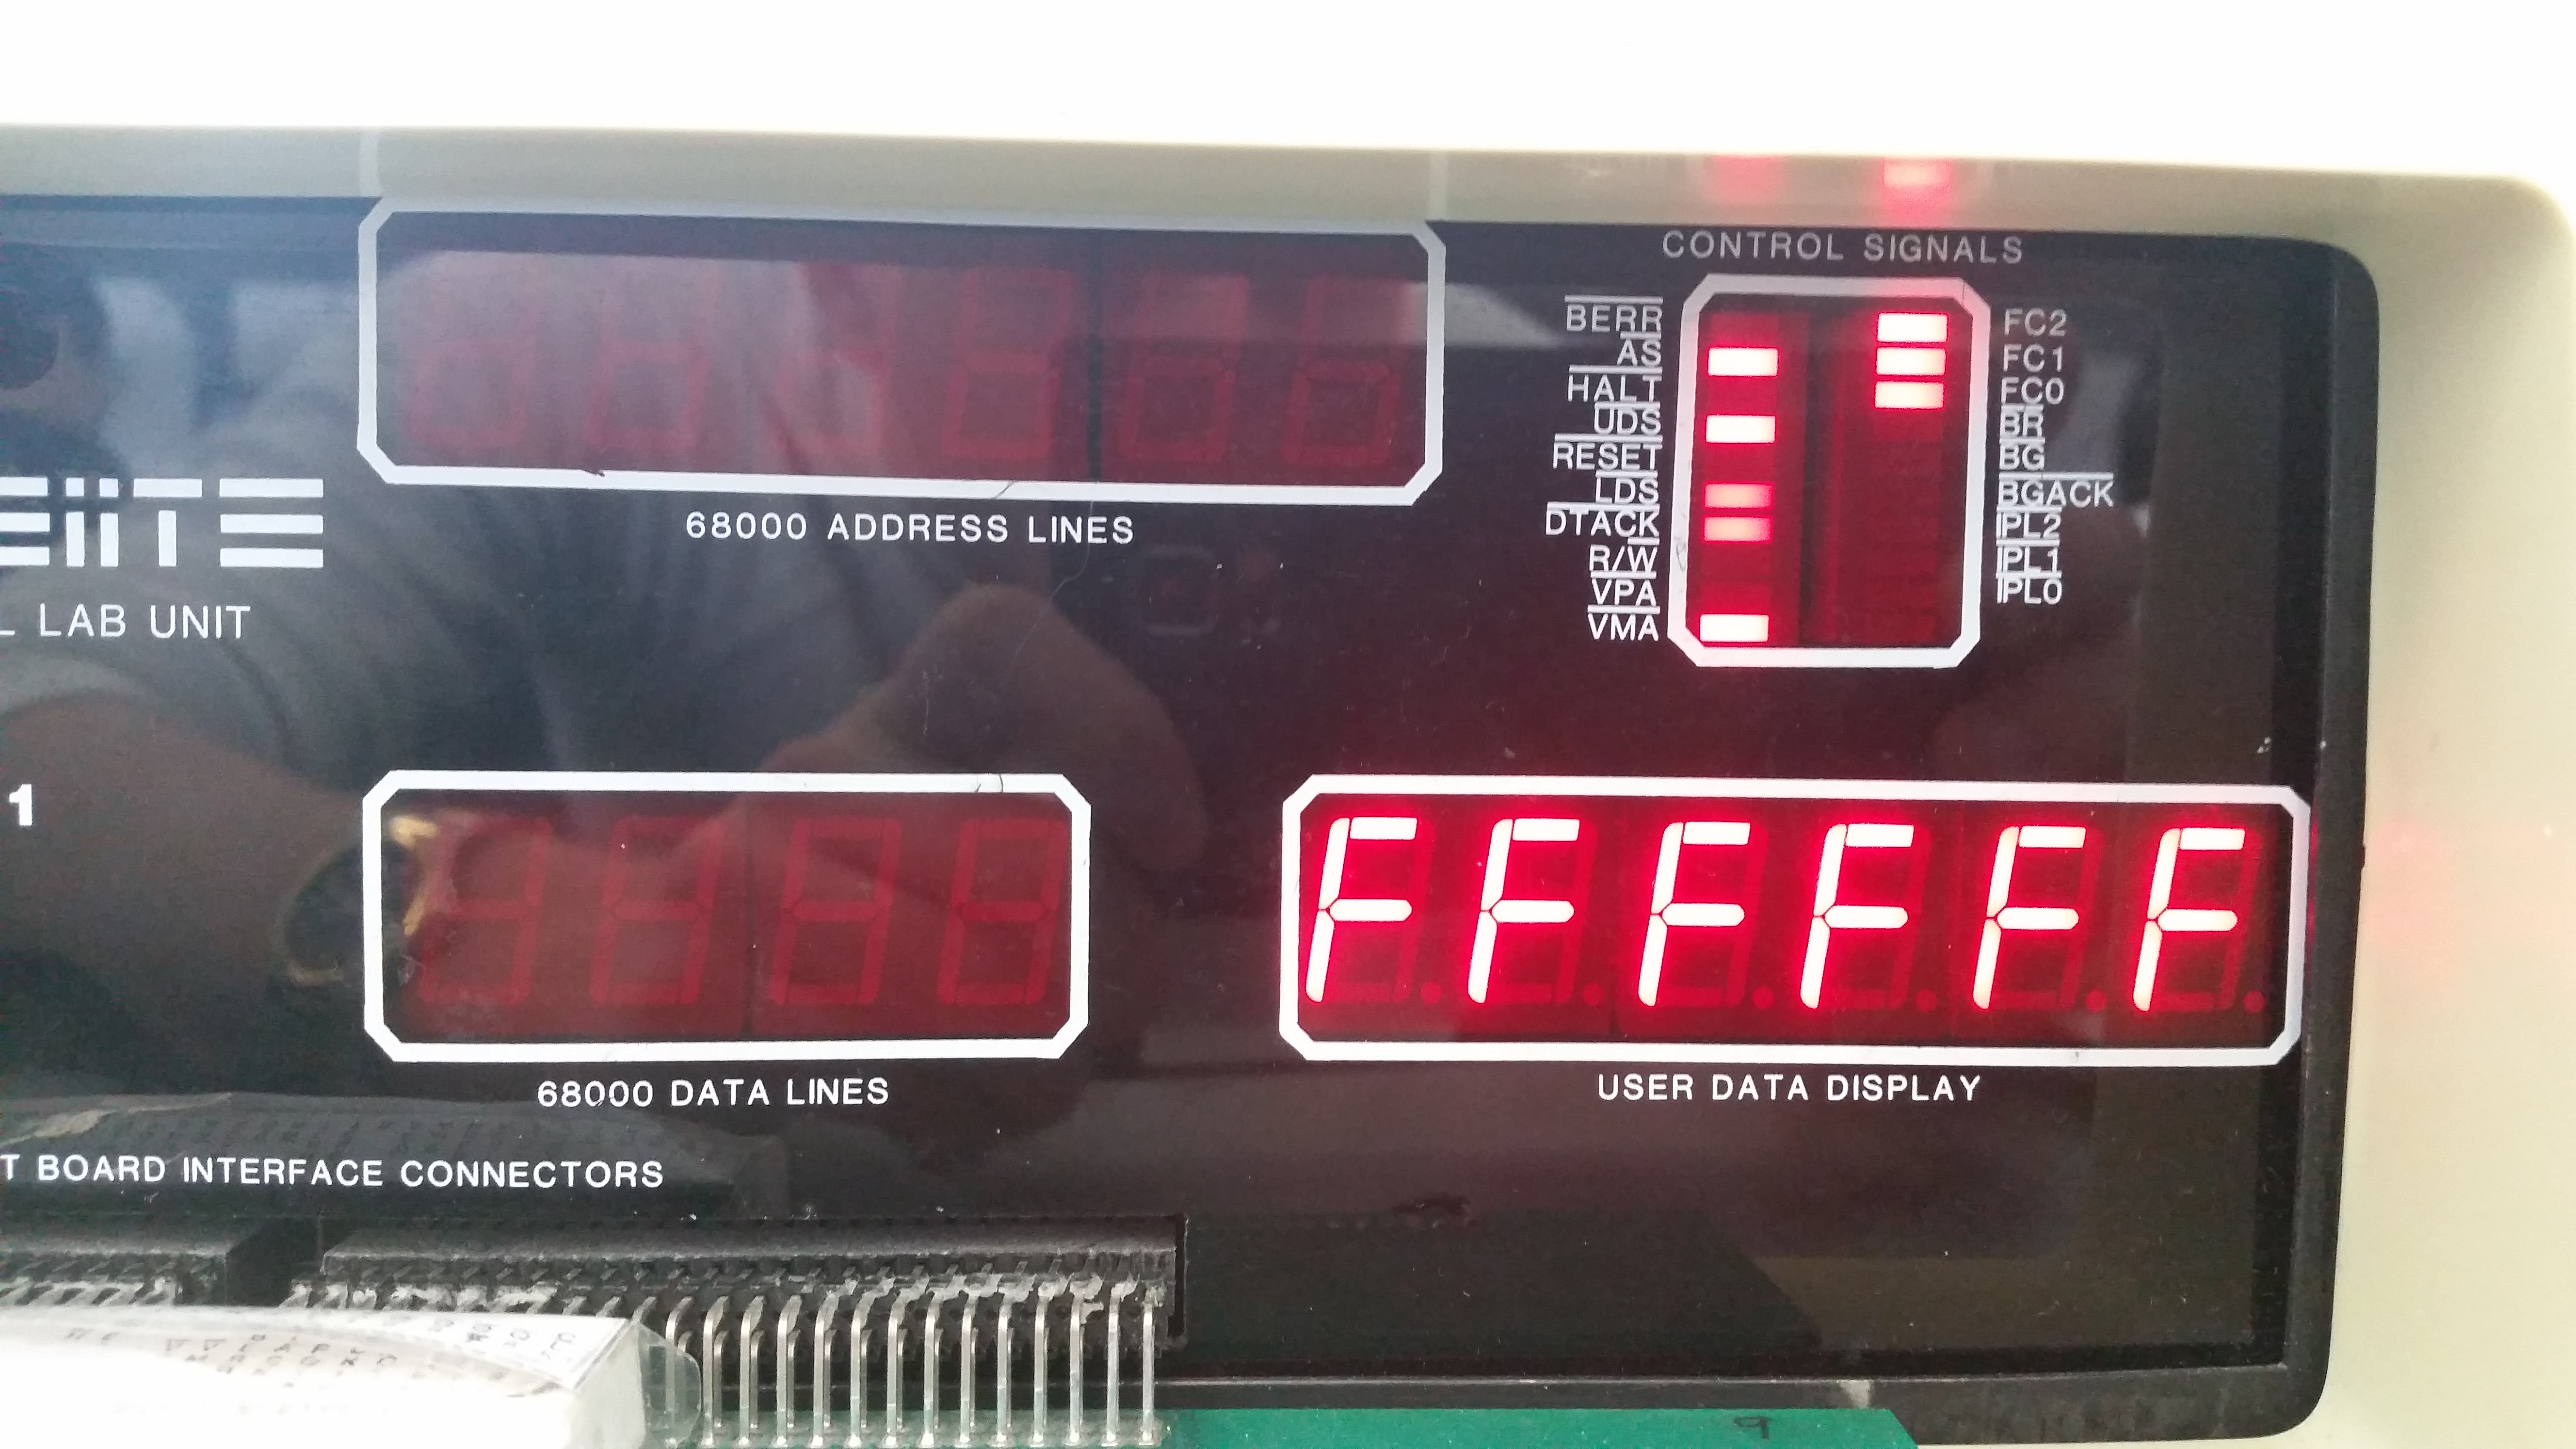
\includegraphics[width=1\linewidth]{20150203_094134}
\caption{State After Pressing the Reset Button}
\label{fig:reset}
\end{figure}

\section{Discussion}
\subsection{Analysis}
Several exception types were explored and analyzed over the coarse of this experiment. They were each successfully invoked and the cause to their invocation was explored. Overall, the results obtained matched the expected results. Refer to Section \ref{questions} for an in depth analysis of each exception/program.
\subsection{Answers to Follow Up Questions}\label{questions}
All code with global and local comments are listed in the Appendix in Section \ref{code}.
\subsubsection{Program 1A}
\begin{enumerate}
	\item Describe how and why the above Address Trap exception occurred.
	\subitem \hspace{-0.7cm}\textbf{Answer:} The address trap exception occurred because the processor attempted to access a word at an odd address location. D0 was loaded with 0xFF, which is an odd address, thus provoking the exception.
\end{enumerate}
\subsubsection{Program 1B}
\begin{enumerate}
	\item Describe how and why the Bus Trap Error exception occurred, and at what instruction.
	\subitem \hspace{-0.7cm}\textbf{Answer:} The bus trap exception occurred because address \$FFFFFF is a nonexistent address. When the processor tried to access it, the bus trap error exception was called.
\end{enumerate}
\subsubsection{Program 1C}
\begin{enumerate}
	\item Describe why the Illegal Instruction exception occurred. What is the purpose of the \$4AFA instruction? List any other opcodes, instructions, etc., which cause this exception to occur.
	\subitem \hspace{-0.7cm}\textbf{Answer:} An illegal instruction refers to any word bit pattern that does not match the bit pattern of the first word of a legal M68000 instruction. There are three bit patterns that always force an illegal instruction trap exception. These patterns are \$4AFA, \$4AFB, and \$4AFC. \$4AFA and \$4AFB are reserved for Motorola system products while \$4AFC is reserved for customer use.
\end{enumerate}
\subsubsection{Program 1D}
\begin{enumerate}
	\item Describe how and why the Privilege Violation exception occurred.
	\subitem \hspace{-0.7cm}\textbf{Answer:} AND-ing an immediate value with the status register is a privileged instruction. Because the processor was running in user mode, this instruction could not be executed and the exception occurred.
\end{enumerate}
\subsubsection{Program 1E}
\begin{enumerate}
	\item Describe how and why the above Zero Divide exception occurred.
	\subitem \hspace{-0.7cm}\textbf{Answer:} An unsigned divide instruction forces an exception if a division operation is attempted with a divisor by zero. D1 contained the value 0 which caused the instruction to invoke the exception.
	\item When performing a division operation and an overflow condition occurs, will exception processing occur? If yes, describe which exception occurs. If no, describe a method for invoking an exception for overflow conditions.
	\subitem \hspace{-0.7cm}\textbf{Answer:} Exception processing will not occur but the overflow bit will be set in the status register. To invoke an exception for overflow conditions, the TRAPV instruction can be used.
\end{enumerate}
\subsubsection{Program 1F}
\begin{enumerate}
	\item Describe how and why the CHK Instruction exception occurred. Describe the advantages of the CHK Instruction.
	\subitem \hspace{-0.7cm}\textbf{Answer:} The CHK instruction checks if the value of the specified address is within the range from 0 to the value of the effective address. Register D7 contained \$3010 while D6 contained \$3000, and since \$3010 is not within the range of 0-3000, the exception occurred. The CHK instruction can be extremely useful when trying to verify that data makes sense, such as being in the correct range of accepted values.
\end{enumerate}
\subsubsection{Program 1G}
\begin{enumerate}
	\item Describe why the LINE 1010 Emulator exception occurred. What purpose does this exception serve?
	\subitem \hspace{-0.7cm}\textbf{Answer:} According to the MC68K User Manual, word patterns with bits 15-12 equaling 1010 or 1111 are distinguished as unimplemented
	instructions, and separate exception vectors are assigned to these patterns. Bits 15-12 were modified to be 0xA or 1010 in binary, so this exception was thrown.
\end{enumerate}

\subsubsection{Program 1H}
\begin{enumerate}
	\item Describe why the LINE 1111 Emulator exception occurred. What purpose does this exception serve?
	\subitem \hspace{-0.7cm}\textbf{Answer:} As stated previously, word patterns with bits 15-12 equaling 1010 or 1111 are distinguished as unimplemented instructions, and separate exception vectors are assigned to these patterns. Bits 15-12 were modified to be 0xF or 1111 in binary, so this exception was thrown. Opcodes beginning with bit patterns equaling 1111 (line F) are implemented in the MC68020 and beyond as co-processor instructions. These separate vectors allow the operating system to emulate unimplemented instructions in software.
\end{enumerate}

\subsubsection{Program 2}
\begin{enumerate}
	\item If you were writing your own Bus Error Exception routine, what type of functions or features would you include in your routine and why?
	\subitem \hspace{-0.7cm}\textbf{Answer:} I'd include the ability to debug, including printouts of locations and context of the error as well as being able to drop into TRACE mode. Essentially, it would be an implementation of GDB. I've found programs like GDB to be extremely useful, especially when running code and only getting SEG-FAULT as the information to why the program crashed.
	\item Explain why the string 'A BUS ERROR JUST OCCURRED' didn’t appear on the screen after the program was executed a second time.
	\subitem \hspace{-0.7cm}\textbf{Answer:} When the entire system was reset, the bus error vector was reset to its default location in memory, so there was no longer a pointer to the user's custom code.
\end{enumerate}
\subsubsection{Program 3}
\begin{enumerate}
	\item With regard to this sample program, describe in detail the sequence of events, which caused the 68000 to enter its HALTED state.
	\subitem \hspace{-0.7cm}\textbf{Answer:} Essentially, a double bus fault occurred. First, the program generated a bus error, however, the bus error exception vector was modified by the user to go to address 0xFFFFFE. When the processor tried to load the address, the second bus error exception was generated. The processor is designed so that if two bus errors are generated, it will HALT the system to prevent any damage to the system.
	\item In general, what sequences of events causes a double bus fault to occur?
	\subitem \hspace{-0.7cm}\textbf{Answer:} Two consecutive bus errors generally incite the exception to occur. This means that there could be faulty error handling code, or a hardware problem.
	\item Describe what effect a double bus error condition has on the 68000’s HALT signal. Discuss the advantages and disadvantages of this feature.
	\subitem \hspace{-0.7cm}\textbf{Answer:} The double bus fault asserts the HALT signal. The advantage is that halting the system can potentially save it from severe damage, however, the disadvantage is that the system must be manually rebooted to continue use.
	\item Describe the result of depressing the ABORT switch and explain the reason for this.
	\subitem \hspace{-0.7cm}\textbf{Answer:} The abort button simply aborts the current execution of code. Since the processor was in a HALT state, nothing happened since no code was being run.
	\item Describe the result of depressing the RESET switch and explain the reason for this.
	\subitem \hspace{-0.7cm}\textbf{Answer:} The reset switch restarted the system. It resets the processor and resets the vector tables. This is why the system was fully functional afterwards.
	\item Explain the differences between the RESET and ABORT switches. Under what conditions would you use the ABORT switch? When you reset the lab unit, what happens to the contents of the Exception Vector Table?
	\subitem \hspace{-0.7cm}\textbf{Answer:} The abort button simply aborts the currently running code and returns to TUTOR. The Reset button aborts the code, resets the processor and resets the vector tables, essentially restarting the system. The abort switch is used to stop execution of code, such as an infinite loop. As stated above, when the lab unit is reset, the exception vector tables are set back to default.
	\item What are the differences between manually activating the RESET pushbutton, and having the 68000 execute the RESET instruction?
	\subitem \hspace{-0.7cm}\textbf{Answer:} According to the 68k instruction set, when the reset instruction is executed, it asserts the RSTO signal for 512 clock periods, resetting all external devices. The processor state, other than the program counter, is unaffected, and execution continues with the next instruction. This instruction has no effect on the processor itself, so the only way to reset it is through the physical reset switch.
\end{enumerate}


\section{Conclusion} 
Overall, this experiment was a success. MC68K Exception Processing, TUTOR Exception Handling, and MC68K system controls were all introduced to the student. From here, the student can utilize the knowledge of exception handling to work on more complex programs involving the \textsc{sanper-1 elu.}
\onecolumn
\section{Appendix}
\label{appendix}
\subsection{Code}\label{code}
\lstset{language=[Motorola68k]Assembler}
\subsubsection{Program 1A}\label{prog1A}
\lstinputlisting{3_1.X68}
\subsubsection{Program 1B}\label{prog1B}
\lstinputlisting{3_1B.X68}
\subsubsection{Program 1D}\label{prog1D}
\lstinputlisting{3_1D.X68}
\subsubsection{Program 1E}\label{prog1E}
\lstinputlisting{3_1E.X68}
\subsubsection{Program 1F}\label{prog1F}
\lstinputlisting{3_1F.X68}
\subsubsection{Program 2}\label{prog2}
\lstinputlisting{3_2.X68}
\subsubsection{Program 2-4}\label{prog2-4}
\lstinputlisting{3_2_4.X68}
\subsubsection{Program 2-12}\label{prog2-12}
\lstinputlisting{3_2_12.X68}
\subsubsection{Program 3}\label{prog3}
\lstinputlisting{3_3.X68}
\begin{thebibliography}{1}
\bibitem{expman} Experiment 3 Lab Manual
\bibitem{ecbm} Educational Computer Board Manual
\bibitem{m68k}MC68K User Manual
\bibitem{sanper}SANPER-1 ELU User Manual


\end{thebibliography}

\end{document}